%\documentclass[10pt]{beamer}
\documentclass[xcolor={pdftex,dvipsnames,table}]{beamer}

\definecolor{redUnipd}{HTML}{9b0014}
\definecolor{grayUnipd}{HTML}{444F51}
\definecolor{myblue}{HTML}{317a9b}
%\definecolor{Black}{RGB}{0,62,114}
\newcommand{\bbf}[1]{\textcolor{black}{\bf #1}}
\newcommand{\rbf}[1]{\textcolor{redUnipd}{ #1}}
\usefonttheme{structurebold}
\usecolortheme[named=myblue]{structure}
\setbeamercolor{structure}{fg=redUnipd}
\setbeamercolor{normal text}{bg=white,fg=grayUnipd}
\setbeamertemplate{itemize items}{$\circ$}
%\textopenbullet
%\usepackage{marvosym}
%\setbeamertemplate{itemize items}{$\Neutral$}

\usepackage{pgfpages}
\pgfpagesuselayout{resize to}[a4paper, 
                                border shrink=1.5cm,
                                landscape]


\usepackage[T1]{fontenc}
%
\usepackage[english]{babel}
\usepackage{graphicx}
\usepackage{booktabs}
\usepackage{latexsym}
\usepackage{subfigure}
\usefonttheme{professionalfonts}
%\usepackage{enumitem}
\usepackage{amsmath,amssymb}
\usepackage[latin1]{inputenc}
%\setbeamercovered{dynamic}
\usepackage{Sweave}
\usepackage[english]{babel}
\usepackage{tikz,comment,amssymb}
\usetikzlibrary{shapes}

\newcommand{\bb}[1]{\begin{block}{#1}}
\newcommand{\eb}{\end{block}}
\newcommand{\bi}{\begin {itemize}}
\newcommand{\ei}{\end{itemize}}
\newcommand{\be}{\begin {enumerate}}
\newcommand{\ee}{\end{enumerate}}
\linespread{1.05}

\newcommand{\bfr}[1]{\begin{frame} \frametitle{#1}}

\AtBeginSection[] {
  \begin{frame}<beamer>
    \frametitle{Outline}
    \tableofcontents[currentsection]
  \end{frame}
}


\title[]{Controllo della Molteplicit\`a nei trial clinici}
\subtitle{FamilyWise Error Rate}
\author[\hspace{5cm}]{Livio Finos}
\date{}
% \date{A.A. 2015/2016 }
%\logo{\includegraphics[scale=.05]{figures/logoUnipd.jpg}}

\begin{document}

\begin{frame}
  \titlepage
\end{frame}

\begin{frame}
Ringrazio i professori Aldo Solari, Jelle Goeman e Florian Klinglmueller per le idee e il materiale condivisi in tutti questi anni. Questo materiale ne \`e una elaborazione.
\end{frame}

% \section{FamilyWise Error Rate (FWER)}
\section{Definizione}

\bfr{FamilyWise Error Rate (FWER)}
\bb{Probabilit\`a di fare ALMENO un falso rifiuto}
  \eb

\begin{eqnarray*}
    \mathrm{FWER} &=& P \big(p_i \leq \widetilde{\alpha}\ per\ almeno\ una\ ipotesi\ i\ nulla\ vera \big) \\
    &=& \mathrm{P} \Big( \bigcup_{i\in \{ipotesi\ nulle\ vere\}} \{p_i \leq \widetilde{\alpha}\} \Big) \\
    \end{eqnarray*}

\end{frame}



\bfr{Correzione di \v{S}id\`ak }
Se voglio controllare il $FWER$ a livello $\alpha$, a quale livello individuale $\widetilde{\alpha}$ devo rifiutare i singoli test?

\begin{eqnarray*}
    \mathrm{FWER}= \alpha &=& P \big(p_i \leq \widetilde{\alpha}\ per\ almeno\ una\ ipotesi\ nulla\ vera \big) = \\
    &=& \mathrm{P} \Big( \bigcup_{i\in \{ipotesi\ nulle\ vere\}} \{p_i \leq \widetilde{\alpha}\} \Big) =\\
    &=& 1 - \mathrm{P} \Big( \bigcap_{i\in \{ipotesi\ nulle\ vere\}} \{p_i > \widetilde{\alpha}\} \Big) = \\
    &&(de Morgan)\\
    &=& 1 - (1- \widetilde{\alpha})^{m_0}= (m_0: \textrm{\#\{ipotesi nulle vere\}}) \\
    && (\textrm{non conosciamo $m_0$, sappiamo che per\`o $m_0\leq m$})\\
    &\leq& 1 - (1- \widetilde{\alpha})^{m} 
    \end{eqnarray*}


\end{frame}

\bfr{Correzione di \v{S}id\`ak }
Da cui ricaviamo:

\begin{eqnarray*}
    1- \alpha &=& (1- \widetilde{\alpha})^{m} \\
    (1- \alpha)^{1/m} &=& (1- \widetilde{\alpha}) \\
  \widetilde{\alpha} &=& 1- (1- \alpha)^{1/m} 
    \end{eqnarray*}

Quindi basta rifiutare ogni singola ipotesi a livello $\widetilde{\alpha} = 1- (1- \alpha)^{1/m}$ (cio\`e rifiuto i p-value per i quali $p \leq \widetilde{\alpha}$)\\
\bigskip
\pause
Purtroppo questa soluzione \`e valida solo quando i p-value sono INDIPENDENTI.
Nella maggior parte dei casi i test hanno una dipendenzza indotta dalla dipendenza tra le variabili originali.

\end{frame}

%\bfr{P-values}
%  \bb{Start from p-values}
%    Often p-value $p_1,\ldots,p_m$ for each hypothesis available
%  \eb
%  \bb{Marginal property}
%    P-values are uniformly distributed under the null hypothesis:\\
%    $\mathrm{P}(p_i \leq \alpha) = \alpha$ if $H_i$ true (sometimes $\leq \alpha$)
%  \eb
%  \bb{Joint distribution}
%    Joint distribution of p-values (dependence) often unknown
%  \eb
%\end{frame}


\bfr{P-values Dipendenti}
Pu\`o capitare che $P(\textrm{Almeno\ un\ Falso\ Rifiuto di } H_0) > (!) 1- (1-\alpha)^2$
\begin{center}
\includegraphics[width=0.5\textwidth]{plaatjes/bivaH0dep}
\end{center}

Remark: ricordate per\`o che le distribuzioni marginali sono uniformi perch\`e i due test sono sotto $H_0$.



\end{frame}




% \section{Bonferroni, Holm and Shaffer}
\section{Bonferroni (single-step)}


\bfr{Boole}
  \bb{Diseguagliansa di Boole}
    Dai due  eventi $A$ e $B$:
    \[ \mathrm{P}(A \cup B) = \mathrm{P}(A) + \mathrm{P}(B) - \mathrm{P}(A \cap B) \]
    e quindi
    \[ \mathrm{P}(A \cup B) \leq \mathrm{P}(A) + \mathrm{P}(B) \]
    Generalizzando al pi\`u eventi $A_1, \ldots, A_m$:
    \[ \mathrm{P}(\bigcup_{i=1}^m A_i) \leq \sum_{i=1}^m \mathrm{P}(A_i) \]
  \eb
  \bb{Equality}
    L'uguaglianza si verifica quando gli eventi sono disgiunti
  \eb
  % \bb{Nessuna assumptione}
  %   Sempre valida
  % \eb
\end{frame}


\bfr{FamilyWise Error Rate (FWER)}
\bb{Probabilit\`a di fare ALMENO un falso rifiuto}
  \eb


\bb{Diseguaglianza di Bonferroni}
     {Riduce $\alpha$} \\
    Rifiuta $H_i$ se $p_i \leq \widetilde{\alpha} =\alpha/m$ ($m=$ numero di ipotesi)
\eb
  \bb{Controllo del FWER}
    \begin{eqnarray*}
    \mathrm{FWER} &=& P \big(p_i \leq \alpha/m\ per\ almeno\ una\ ipotesi\ i\ nulla\ vera \big) \\
    &=& \mathrm{P} \Big( \bigcup_{i\in \{ipotesi\ nulle\ vere\}} \{p_i \leq \alpha/m\} \Big) \\
    &\leq& \sum_{i \in \{ipotesi\ nulle\ vere\}} \mathrm{P} (p_i \leq \alpha/m) \\
    &\leq& m_0\frac{\alpha}{m} \leq \alpha
    \end{eqnarray*}
  \eb
\end{frame}
% 
% 
% \bfr{The Bonferroni inequality}
%  \bb{Reduced $\alpha$}
%    Bonferroni: reduce significance level for each hypothesis
%    \\ Rifiuta $H_i$ if $p_i \leq \alpha/m$
%  \eb
%  \bb{Control of FWER}
%    \begin{eqnarray*}
%    \mathrm{FWER} &=& \mathrm{P} \big(\textrm{$p_i \leq \alpha/m$ for at least one $i$ with $H_i$ true} \big) \\
%    &=& \mathrm{P} \Big( \bigcup_{i\in T} \{p_i \leq \alpha/m\} \Big) \\
%    &\leq& \sum_{i \in T} \mathrm{P} (p_i \leq \alpha/m) \\
%    &\leq& \#T\frac{\alpha}{m} \leq \alpha
%    \end{eqnarray*}
%  \eb
% \end{frame}
% 


%%%%%%%%%%%%%%%%%BUONO PER MASTER, sostituiscono la successiva:
%%%%%%%%%%%%%%%%%BUONO PER MASTER, sostituiscono la successiva:
%%%%%%%%%%%%%%%%%BUONO PER MASTER, sostituiscono la successiva:
%%%%%%%%%%%%%%%%%BUONO PER MASTER, sostituiscono la successiva:
%%%%%%%%%%%%%%%%%BUONO PER MASTER, sostituiscono la successiva:
%%%%%%%%%%%%%%%%%BUONO PER MASTER, sostituiscono la successiva:
%%%%%%%%%%%%%%%%%BUONO PER MASTER, sostituiscono la successiva:
%%%%%%%%%%%%%%%%%BUONO PER MASTER, sostituiscono la successiva:
% \bfr{Using Bonferroni}
%  \bb{Advantages}
%    \bi
%      \item Extremely easy
%      \item Strong control of FWER under any dependence of p-values
%    \ei
%  \eb
%  \bb{Disadvantage}
%    Conservative: FWER $\leq \alpha$, often $<\alpha$
%  \eb
%  \bb{When is Bonferroni least conservative?}
%    \bi
%      \item Events $\{p_i \leq \alpha/m\}$ disjoint
%      \item $\# T = m$: complete null hypothesis
%    \ei
%  \eb
% \end{frame}
% 



\bfr{Procedura di Bonferroni}
 \bb{Multiplicity adjusted p-value}
    $\tilde p_i = mp_i$ $i=1,\ldots,m$ e rifiuta se  $\leq \alpha$
  \eb
  \bb{Vantaggi}
    \bi
      \item Molto facile
      \item Controlla il FWER sotto ogni dipendenza
    \ei
  \eb
  \bb{Svantaggi}
    Conservativo (Adj. p-value molto alti, pochi rifiuti)
  \eb
\end{frame}


\section{Holm (step-wise)}

\bfr{Holm's procedure\footnote{Holm S. (1979) A simple sequentially rejective multiple test procedure. {\it Scandinavian Journal of Statistics}; 6(2):65--70.}}
%\textcolor{redUnipd}{$\quad$\textbf{Holm's sequential procedure}}


\begin{enumerate}
\item Primo passo: adjusted p-value: $p\cdot m$; rifiuta se $\leq \alpha$
\item Dopo $r$ rifiuti, adjusted p-value: $p\cdot (m-r)$
\item Stop appena non rifiuti nulla
\end{enumerate}

\begin{center}
\begin{overprint}
\only<1>{\bbf{Bonferroni}}
\only<2>{\bbf{Supponiamo $p_A$ e $p_C$ significativi}}
\only<3>{\bbf{Adjusted p-value: $p\cdot 3$}}
\only<4>{\bbf{Supponamo $p_D$ significativo}}
\only<5>{\bbf{Adjusted p-value: $p\cdot 2$}}
\only<6>{\bbf{Nessun rifiuto. Stop}}
\begin{tikzpicture}
\node at (-.4,1) {$\mathcal{H}\setminus \mathcal{R}:$};
\node at (0,0) {$\mathcal{R}:$};
\node at (-1,2) {Adj. p-value:};
\node at (6,2) {\bbf{$\leq ? \alpha$}};
\only<1>{
\node at (1,2) {$p_A 5$};
\node at (2,2) {$p_B 5$};
\node at (3,2) {$p_C 5$};
\node at (4,2) {$p_D 5$};
\node at (5,2) {$p_E 5$};
\draw[] 
(1,1) node[draw, line width=1pt,fill=black!50] {A}
(2,1) node[draw, line width=1pt,fill=black!50] {B}
(3,1) node[draw, line width=1pt,fill=black!50] {C}
(4,1) node[draw, line width=1pt,fill=black!50] {D}
(5,1) node[draw, line width=1pt,fill=black!50] {E};}
\only<2>{
\node at (1,2) {$p_A 5$};
\node at (2,2) {$p_B 5$};
\node at (3,2) {$p_C 5$};
\node at (4,2) {$p_D 5$};
\node at (5,2) {$p_E 5$};
\draw[] 
(1,1) node[draw, line width=1pt,fill=redUnipd!90] {A}
(2,1) node[draw, line width=1pt,fill=black!50] {B}
(3,1) node[draw, line width=1pt,fill=redUnipd!90] {C}
(4,1) node[draw, line width=1pt,fill=black!50] {D}
(5,1) node[draw, line width=1pt,fill=black!50] {E};}
\only<3>{
\node at (1,2) {-};
\node at (2,2) {$p_B3$};
\node at (3,2) {-};
\node at (4,2) {$p_D3$};
\node at (5,2) {$p_E3$};
\draw[] 
(1,0) node[draw, line width=1pt,fill=redUnipd!90] {A}
(2,1) node[draw, line width=1pt,fill=black!50] {B}
(3,0) node[draw, line width=1pt,fill=redUnipd!90] {C}
(4,1) node[draw, line width=1pt,fill=black!50] {D}
(5,1) node[draw, line width=1pt,fill=black!50] {E};}
\only<4>{
\node at (1,2) {-};
\node at (2,2) {$p_B3$};
\node at (3,2) {-};
\node at (4,2) {$p_D3$};
\node at (5,2) {$p_E3$};
\draw[] 
(1,0) node[draw, line width=1pt,fill=redUnipd!90] {A}
(2,1) node[draw, line width=1pt,fill=black!50] {B}
(3,0) node[draw, line width=1pt,fill=redUnipd!90] {C}
(4,1) node[draw, line width=1pt,fill=redUnipd!90] {D}
(5,1) node[draw, line width=1pt,fill=black!50] {E};}
\only<5-6>{
\node at (1,2) {-};
\node at (2,2) {$p_B2$};
\node at (3,2) {-};
\node at (4,2) {-};
\node at (5,2) {$p_E2$};
\draw[] 
(1,0) node[draw, line width=1pt,fill=redUnipd!90] {A}
(2,1) node[draw, line width=1pt,fill=black!50] {B}
(3,0) node[draw, line width=1pt,fill=redUnipd!90] {C}
(4,0) node[draw, line width=1pt,fill=redUnipd!90] {D}
(5,1) node[draw, line width=1pt,fill=black!50] {E};}
\end{tikzpicture}
\end{overprint}
\end{center}
\end{frame}


%%%%%%%%%%%%%%%%%
%\bfr{Risultati Holm}
%%p.adjust(c(.217,.0015,.0072,.0001,.0415,.0025,.3545,.0189, .1264 ,.5856, .5536, 1.000),"holm")
%% [1] 1.0000 0.0165 0.0648 0.0012 0.2905 0.0250 1.0000 0.1512 0.7584 1.0000 1.0000 1.0000
%\begin{small}
%\begin{center}
%\begin{tabular}{ l | c  | r c}
% & p-value & Adjusted p-value & \\
%\hline
%%ECRR & & &\\
%ECRR: Ansia&.217 & 1.000& \\
%ECRR: Evitamento&.0015 & .0165 & *\\
%\hline
%%DAS & & \\
%DAS: Consenso&.0072& .0648 & \\
%DAS: Soddisfazione&.0001&  .0012 & *\\
%DAS: Coesione&.0415& .2905 & \\
%DAS: Espr.Affetti&.0025& .0250 & *\\
%\hline
%%AAI & & \\
%AAI: Sicuro & .3545 & 1.000\\
%AAI: Distanziante & .0189& .1512 & \\
%AAI: Preoccupato & .1264 & .7584 & \\
%\hline
%%CRI& & \\
%CRI: Sicuro & .5856 & 1.000 & \\
%CRI: Distanziante & .5536 & 1.000 & \\
%CRI: Preoccupato & 1.000 & 1.000 & \\
%%\hline
%\end{tabular}
%\end{center}
%\end{small}
%\end{frame}
%%%%%%%%%%%%%%%%%%%%%%%%%%%%%%%%%%%%%%%%%%%%%%%%%%%%%%%%%%%%%%%%%%%%%%%%%%%%%%%%%%%%%%%%%%%%%%%%%%%%%%
\section{Closed Testing}
\begin{frame}
\frametitle{Closed Testing\footnote{R Marcus, E Peritz, KR Gabriel (1976). On closed testing procedures with special reference to ordered analysis of variance. Biometrika 63: 655-660.}}
\begin{overprint}
\only<1>{Insieme Chiusura delle ipotesi (tutte le possibili intersezioni)}
\only<2>{Test nodo superiore (es MANOVA)}
\only<9>{\bbf{ Svantaggio: ipotesi testate diventano sono spesso troppe: $=2^{\# ipotesi}-1$}}
\end{overprint}
\begin{center}
\only<1>{\bbf{Ipotesi iniziali}}
\only<2>{\bbf{Insieme chiusura}}
\only<3>{\bbf{Test il nodo principale a livello $\alpha$}}
\only<4>{\bbf{Supponiamo sia significativo}}
\only<5>{\bbf{Avanti}}
\only<6>{\bbf{Verifica i successivi a livello $\alpha$}}
\only<7>{\bbf{Avanti}}
\only<8-9>{\bbf{Identifica i significativi}}
\medskip

\begin{tikzpicture}
\only<1>{
\draw[] 
(0,4) node[draw, color=white] {A}
(-2,0) node[draw, line width=1pt] {A}
(0,0) node[draw, line width=1pt] {B}
(2,0) node[draw, line width=1pt] {C};
}
\only<2>{
\draw[] 
(0,4) node[draw, line width=1pt] {ABC}
(-1.5,2) node[draw, line width=1pt] {AB}
(0,2) node[draw, line width=1pt] {AC}
(1.5,2) node[draw, line width=1pt] {BC}
(-2,0) node[draw, line width=1pt] {A}
(0,0) node[draw, line width=1pt] {B}
(2,0) node[draw, line width=1pt] {C};
}
\only<3>{
\draw[] 
(.8,4) node {$\alpha$}
(0,4) node[draw, line width=1pt,fill=black!50] {ABC}
(-1.5,2) node[draw, line width=1pt] {AB}
(0,2) node[draw, line width=1pt] {AC}
(1.5,2) node[draw, line width=1pt] {BC}
(-2,0) node[draw, line width=1pt] {A}
(0,0) node[draw, line width=1pt] {B}
(2,0) node[draw, line width=1pt] {C};
}
\only<4>{
\draw[] 
(.8,4) node {-}
(0,4) node[draw, line width=1pt,fill=redUnipd!90] {ABC}
(-1.5,2) node[draw, line width=1pt] {AB}
(0,2) node[draw, line width=1pt] {AC}
(1.5,2) node[draw, line width=1pt] {BC}
(-2,0) node[draw, line width=1pt] {A}
(0,0) node[draw, line width=1pt] {B}
(2,0) node[draw, line width=1pt] {C};
}
\only<5>{
\draw[] 
(.8,4) node {-}
(2.1,2) node {$\alpha$}
(-.9,2) node {$\alpha$}
(.6,2) node {$\alpha$}
(0,4) node[draw, line width=1pt,fill=redUnipd!90] {ABC}
(-1.5,2) node[draw, line width=1pt,fill=black!50] {AB}
(0,2) node[draw, line width=1pt,fill=black!50] {AC}
(1.5,2) node[draw, line width=1pt,fill=black!50] {BC}
(-2,0) node[draw, line width=1pt] {A}
(0,0) node[draw, line width=1pt] {B}
(2,0) node[draw, line width=1pt] {C};
%\draw[->, line width=1pt] (0,3.7) -- (-1.5,2.3);
%\draw[->, line width=1pt] (0,3.7) -- (0,2.3);
%\draw[->, line width=1pt] (0,3.7) -- (1.5,2.3);
}
\only<6>{
\draw[] 
(.8,4) node {-}
(2.1,2) node {$\alpha$}
(-.9,2) node {-}
(.6,2) node {-}
(0,4) node[draw, line width=1pt,fill=redUnipd!90] {ABC}
(-1.5,2) node[draw, line width=1pt,fill=redUnipd!90] {AB}
(0,2) node[draw, line width=1pt,fill=redUnipd!90] {AC}
(1.5,2) node[draw, line width=1pt,fill=black!50] {BC}
(-2,0) node[draw, line width=1pt] {A}
(0,0) node[draw, line width=1pt] {B}
(2,0) node[draw, line width=1pt] {C};
%\draw[->, line width=1pt] (0,3.7) -- (-1.5,2.3);
%\draw[->, line width=1pt] (0,3.7) -- (0,2.3);
%\draw[->, line width=1pt] (0,3.7) -- (1.5,2.3);
}
\only<7>{
\draw[] 
(.8,4) node {-}
(2.1,2) node {$\alpha$}
(-.9,2) node {-}
(.6,2) node {-}
(-1.5,0) node {$\alpha$}
(0,4) node[draw, line width=1pt,fill=redUnipd!90] {ABC}
(-1.5,2) node[draw, line width=1pt,fill=redUnipd!90] {AB}
(0,2) node[draw, line width=1pt,fill=redUnipd!90] {AC}
(1.5,2) node[draw, line width=1pt,fill=black!50] {BC}
(-2,0) node[draw, line width=1pt,fill=black!50] {A}
(0,0) node[draw, line width=1pt] {B}
(2,0) node[draw, line width=1pt] {C};
%\draw[->, line width=1pt] (0,3.7) -- (-1.5,2.3);
%\draw[->, line width=1pt] (0,3.7) -- (0,2.3);
%\draw[->, line width=1pt] (0,3.7) -- (1.5,2.3);
%\draw[->, line width=1pt] (-1.5,1.7) -- (-2,0.3);
%\draw[->, line width=1pt] (0,1.7) -- (-1.7,0.3);
}
\only<8-9>{
\draw[] 
(.8,4) node {-}
(2.1,2) node {$\alpha$}
(-.9,2) node {-}
(.6,2) node {-}
(-1.5,0) node {-}
(0,4) node[draw, line width=1pt,fill=redUnipd!90] {ABC}
(-1.5,2) node[draw, line width=1pt,fill=redUnipd!90] {AB}
(0,2) node[draw, line width=1pt,fill=redUnipd!90] {AC}
(1.5,2) node[draw, line width=1pt,fill=black!50] {BC}
(-2,0) node[draw, line width=1pt,fill=redUnipd!90] {A}
(0,0) node[draw, line width=1pt] {B}
(2,0) node[draw, line width=1pt] {C};
%\draw[->, line width=1pt] (0,3.7) -- (-1.5,2.3);
%\draw[->, line width=1pt] (0,3.7) -- (0,2.3);
%\draw[->, line width=1pt] (0,3.7) -- (1.5,2.3);
%\draw[->, line width=1pt] (-1.5,1.7) -- (-2,0.3);
%\draw[->, line width=1pt] (0,1.7) -- (-1.7,0.3);
}
\end{tikzpicture}
\end{center}
\end{frame}

\section{Combinazioni Ristrette di Ipotesi (Shaffer)}
\bfr{Ipotesi Logicamente relate}
{Combinazioni ristrette (Shaffer)}
 \bb{Esempio}
   Modello Anova. 3 campioni.\\
   Ipothesi: Confronto a coppie dei tre campioni.
   \begin{eqnarray*}
     H_{12}&:& \mu_1=\mu_2\\
     H_{23}&:& \mu_2=\mu_3\\
     H_{13}&:& \mu_1=\mu_3
   \end{eqnarray*}
 \eb
 \bb{Relazioni}
   Se $H_{12}$ \`e falsa, $H_{23}$ e $H_{13}$ non possono essere entrambe vere.
 \eb
 \bb{Combinazioni ristrette}
   Non tutte le combinazioni di ipotesi vere/false sono possibili
 \eb
\end{frame}


\bfr{Procedura di Shaffer}
 \bb{metodo di Holm + combinazioni ristrette}
   Test iniziale $c = \alpha/m$
   \\ Ripeti
   \be
     \item Rifiuta tutte le ipotesi con p-value $\leq c$
     \item Ricalcola $c = \alpha/s$ \\ con $s$ il massimo numero di ipotesi che possono essere contemporaneamente vere assumendo che tutti i rifiuti precedenti sono corretti (ipotesi $H_1$ vera)
   \ee
 \eb
 \bb{Confronto con Holm}
   Metodo valido sotto le stessse assunzioni di Holm
   \\ Meno conservativo di Holm in caso combinazioni ristrette
 \eb
\end{frame}

\bfr{Shaffer: esempio}
 \bb{Ipotesi e p-value ($\alpha=0.05$)}
   \begin{eqnarray*}
     H_{12}&:& \mu_1=\mu_2 \qquad p_{12} = 0.01\\
     H_{23}&:& \mu_2=\mu_3 \qquad p_{23} = 0.04\\
     H_{13}&:& \mu_1=\mu_3 \qquad p_{13} = 0.53
   \end{eqnarray*}
 \eb
 \bb{Procedura di Shaffer}
   \be
     \item Rifiuta tutte $H$ con  $p\leq \alpha/3=.0167$ $\to$ Rifiuta $H_{12}$
     \item Se $H_{12}$ \`e falsa, al pi\`u una tra $H_{23}$ e $H_{13}$ pu\`o essere contemporaneamente vera.
     \item Rifiuta tutte le $H$ con $p\leq \alpha/1$  $\to$ Rifiuta $H_{23}$
     \item Continua:\ldots Nessuno ulteriore rifiuto \`e  possibile.
   \ee
 \eb
\end{frame}


\section{Summary}

\bfr{Summary}
  \bb{FamilyWise Error}
    \bi
      \item Generalizza gli errori di Tipo I al caso di ipotesi multiple 
\pause
      \item Controlla la probabilit\`a di ALMENO un falso tra tutti i rifiuti
\pause
      \item corregge i p-value (adjusted p-value sempre uguale o peggiore dei p-value non aggiustati)
    \ei
  \eb
\pause
  \bb{Software R}
    \bi
      \item Bonferroni e Holm: {\tt library(stats); p.adjust()}
  \item Closed Testing {\tt library(cherry); closed()}
    % \item Ipotesi Strutturate {\tt library(globaltest); inheritance()}
    \item Post-hoc ed altro {\tt library(multcomp); glht()}
  % \item Permutazioni - Westfall \&\ Young\\ {\tt library(flip); flip.adjust()}
    \ei
  \eb
\end{frame}
%%%%%%%%%%%%%%%%%%%%%

\end{document}


